\item {\bf Linear regression: linear in what?}

In the first two lectures, you have seen how to fit a linear function of the data for the regression problem.  In this question, we will see how linear regression can be used to fit non-linear functions of the data using feature maps. We will also explore some of its limitations, for which future lectures will discuss fixes.

\begin{enumerate}
	\input{02-featuremaps/01-degree-3-math}

	\item \points{2b} {\bf Degree-k polynomial regression}


For this sub-question question, we will use the datasets provided in
the following file:
%
\begin{center}
	\texttt{src/train.csv}
\end{center}
%

This file contains two columns: $x$ and $y$. In the terminology described in the introduction, $x$ is the attribute (in this case one dimensional) and $y$ is the output label.

Using the formulation of the previous sub-question, implement linear regression with \textbf{normal equations} using the feature map of degree-k polynomials. Using the |LinearModel| provided in |src/submission.py|, this means you will be implementing the functions |fit()|, |predict()|, |create_poly()|, and |run_exp()|.  

To extend the idea above to degree-$k$ polynomials, consider $\phi:\mathbb{R}\rightarrow \mathbb{R}^{k+1}$ to be 
		\begin{align}
	\phi(x) = \left[\begin{array}{c} 1\\ x \\ x^2\\ \vdots \\x^k \end{array}\right]\in \mathbb{R}^{k+1} \label{eqn:feature-k}
	\end{align}

We will use $k=1,2,3,5,10,20$ as test cases. To verify a correct implementation, autograder test case |2b-9-basic| will create a plot in |src/large-poly.png|.  Note that test |2b-9-basic| will NOT be awarded points and is used to test if your implementation can generate a plot similar to the following:

\begin{figure}[H]
  \centering
  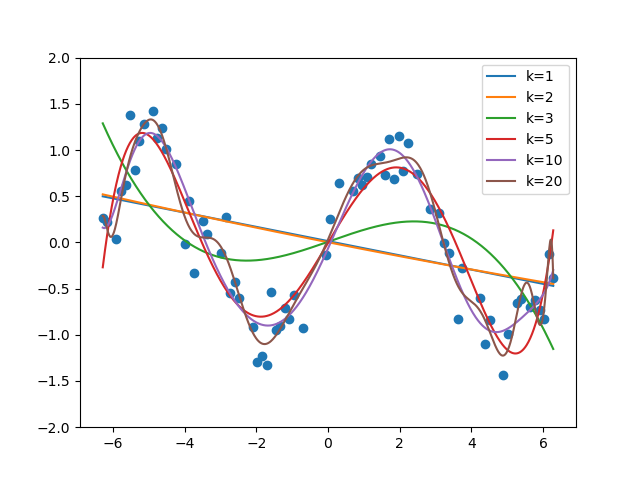
\includegraphics[width=0.65\linewidth]{02-featuremaps/large-poly.png}
  \centering
\caption{Polynomial regression with kernel sizes 1,2,3,5,10 and 20. Visual impaired students can access the corresponding desmos plot \href{https://www.desmos.com/calculator/n7zoh04cfm}{here}}
\end{figure}

  \input{02-featuremaps/03-degree-k-comment}

  \item \points{2d} {\bf Other feature maps}

You may have observed that it requires a relatively high degree $k$ to fit the given training data, and this is because the dataset cannot be explained (i.e., approximated) very well by low-degree polynomials. By visualizing the data, you may have realized that $y$ can be approximated well by a sine wave. In fact, we generated the data by sampling from $y = \sin(x) + \xi$, where $\xi$ is noise with Gaussian distribution. Please update the feature map $\phi$ to include a sine transformation as follows:

\begin{align}
\phi(x) = \left[\begin{array}{c} \sin(x) \\ 1 \\ x \\ x^2\\ \vdots \\x^k\end{array}\right]\in \mathbb{R}^{k+2} \label{eqn:feature-sine}
\end{align}

Complete the function |create_sin()| in |src/submission.py| to implement the updated feature map.  Again, ensure your code  works with a general $k$.  We will use $k=1,2,3,5,10,20$ as test cases. To verify a correct implementation, autograder test case |2d-7-basic| will create a plot in |src/large-sine.png|. Note that test |2d-7-basic| will NOT be awarded points and is used to test if your implementation can generate a plot similar to the following:

\begin{figure}[H]
  \centering
  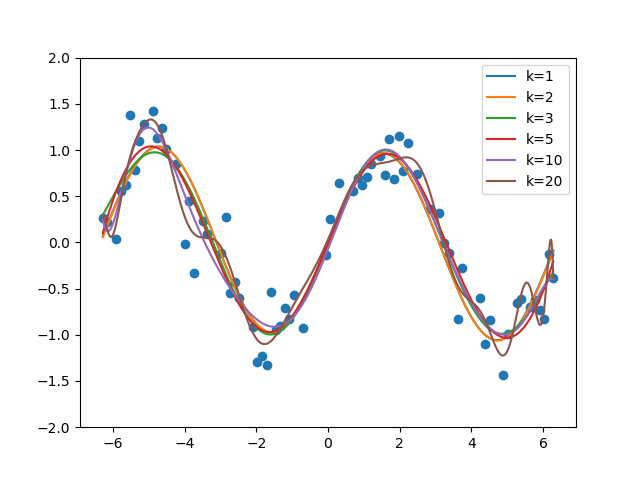
\includegraphics[width=0.65\linewidth]{02-featuremaps/large-sine.png}
  \centering
\caption{Polynomial regression with other features with kernel sizes 1,2,3,5,10 and 20. Visual impaired students can access the corresponding desmos plot \href{https://www.desmos.com/calculator/ikkytcrqyp}{here}}
\end{figure}


  \input{02-featuremaps/05-other-features-comment}

  \item \points{2f} {\bf Overfitting with expressive models and small data}

You will not be required to code, write, or submit anything for this sub-question.  For this and the remaining sub-questions, we will consider a small
dataset (a random subset of the dataset you have been using so far) with much fewer examples, provided in
the following file:
%
\begin{center}
	\texttt{src/small.csv}
\end{center}
%

We will be exploring what happens when the number of features start becoming bigger than the number of 
examples in the training set. Run your algorithm on this small dataset using the following feature map 
\begin{align}
\phi(x) = \left[\begin{array}{c} 1\\ x \\ x^2\\ \vdots \\x^k \end{array}\right]\in \mathbb{R}^{k+1} 
\end{align}
with $k = 1,2,3,5,10,20$ using the autograder test case |2f-0-basic|, which will create plots in |src/smalle-poly.png| and |src/small-sine.png|. 

\textbf{Remark: } The phenomenon you observe where the models start to fit the training dataset very well, but suddenly ``goes wild'' is due to what is called \emph{overfitting}. The intuition to have for now is that, when the amount of data you have is small relative to the expressive capacity of the family of possible models (that is, the hypothesis class, which, in this case, is the family of all degree $k$ polynomials), it results in overfitting.  

Loosely speaking, the set of hypothesis function is ``very flexible'' and can be easily forced to pass through all your data points especially in unnatural ways. In other words, the  model explains the noises in the training dataset, which shouldn't be explained in the first place. This hurts the predictive power of the model on test examples. We will describe overfitting in more detail in future lectures when we cover learning theory and bias-variance tradeoffs.\\

Your plots should look similar to the following:
\begin{figure}[H]
  \centering
  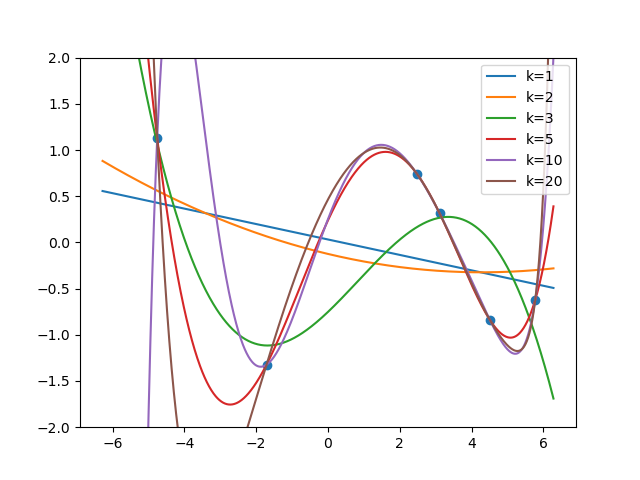
\includegraphics[width=0.65\linewidth]{02-featuremaps/small-poly.png}
  \caption{Polynomial regression with kernel sizes 1,2,3,5,10 and 20
  on small dataset. Visual impaired students can access the corresponding desmos plot \href{https://www.desmos.com/calculator/dwmvngfeyu}{here}}
  
  \centering
  \vspace{2mm}
  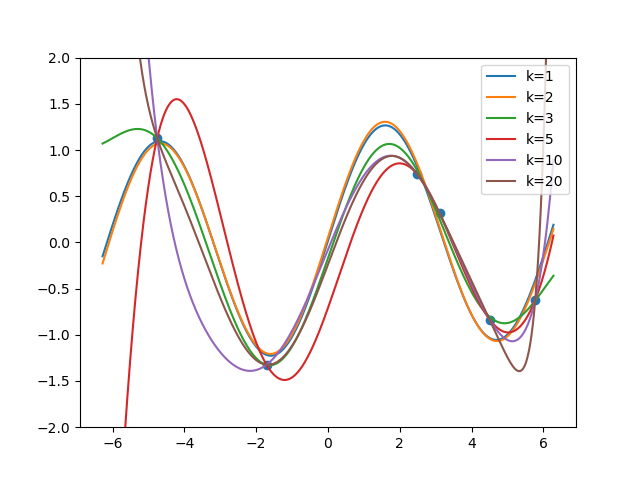
\includegraphics[width=0.65\linewidth]{02-featuremaps/small-sine.png}
  \centering
  \caption{Regression with other polynomial and sinusoidal features with kernel sizes 1,2,3,5,10 and 20
  on small dataset. Visual impaired students can access the corresponding desmos plot \href{https://www.desmos.com/calculator/wb7cepiy6y}{here}}
\end{figure}


  \input{02-featuremaps/07-overfitting-comment}
\end{enumerate}
